\section{Data analysis}
As no data was surveyed by the authors, there will be no chapter on the experimental procedure. Instead, the focus will be on the analysis of the data, for most of which the framework ROOT was used. Data was provided from two sources:
\begin{enumerate}
	\item Monte Carlo simulations, separated by decay reaction.
	\item Actual data from the OPAL detector at the LEP collider.
\end{enumerate}


\subsection{Selection of cuts}
In a first step, the data from the Monte Carlo simulations is plotted over adequate range in the following parameters:
\begin{itemize}
	\item{\makebox[2.5cm][l]{\textbf{NCHARGED:}} The number of tracks visible in the drift chamber}
	\item{\makebox[2.5cm][l]{\textbf{PCHARGED:}} Energy of particles that left a track in the drift chamber}
	\item{\makebox[2.5cm][l]{\textbf{E\_ECAL:}} Energy deposited in the electromagnetic calorimeter}
	\item{\makebox[2.5cm][l]{\textbf{E\_HCAL:}} Energy deposited in the hadronic calorimeter}
	\item{\makebox[2.5cm][l]{\textbf{COS\_THET:}} Angle $\theta$ between created the positive lepton and the \\incident positron beam}
	\item{\makebox[2.5cm][l]{\textbf{COS\_THRU:}} Angle between the thrust axis for hadronic events and the \\incident positron beam}
\end{itemize}
These plots include the simulation events from decays to electrons, myons, tauons as well as quarks in similar amounts. These ratios are not a representation of the actual ratios as they would be expected in the real data, as the decay width of quarks is much greater than that of the three types of leptons. \\
To further improve comparability of the different data sets, all histograms were normed to an integral of 1. The resulting plots are shown in graphics !!ADD GRAPHS REF!!. Using these graphs, as well as the knowledge of the type of event, cuts are established which will later be used to separate the actual data, where there is no initial knowledge of the type of event.\\
Thus, for every type of educts, a cut is to be made with maximum possible efficiency in detecting the respective kind of event, as well as maximum purity, meaning that other events are falsely allotted as rarely as possible.

\newpage
\begin{figure}[h]
\centering
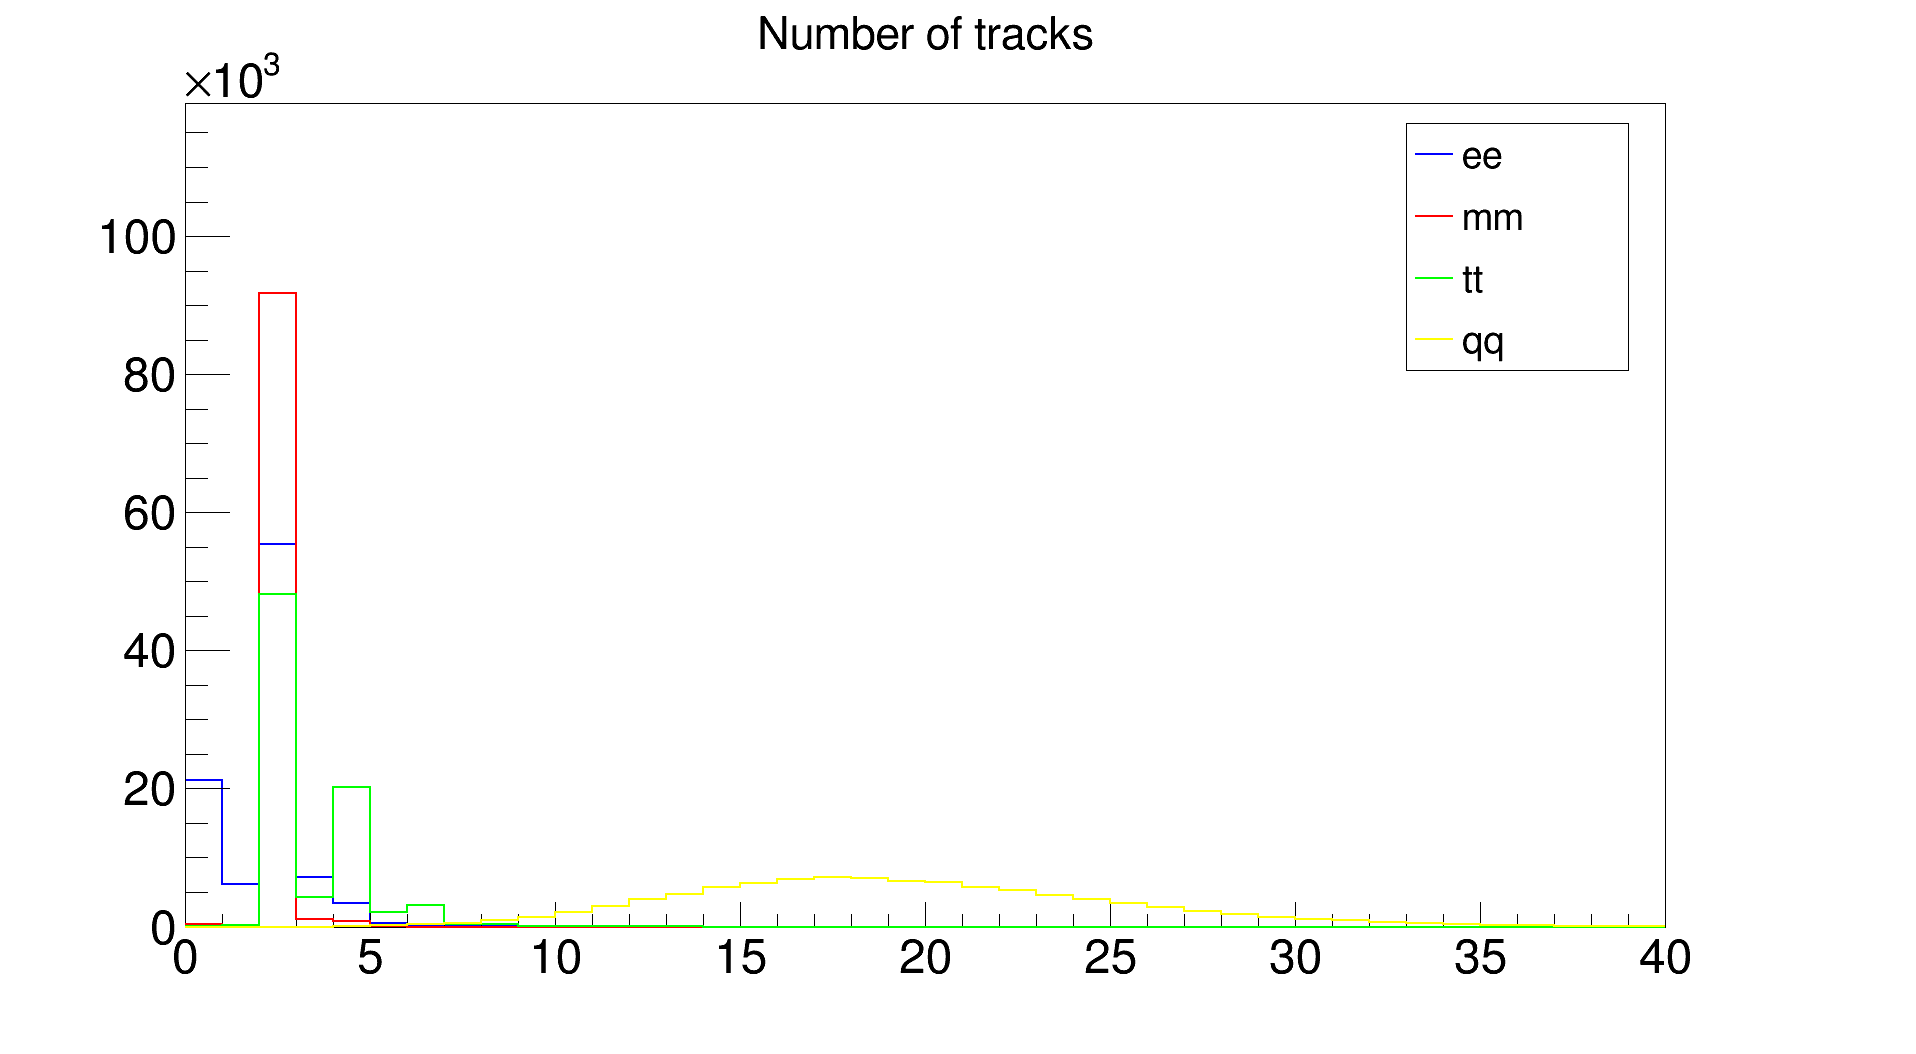
\includegraphics[width=1\linewidth]{../results/MC_results/nocut/Ncharged}
\caption[Ncharged in simulation data]{This figure shows the number of charged tracks in the simulation data. Almost all muon events leave two tracks. The peak is cut off to increase visibility of the other data.}
\label{fig:Ncharged}
\end{figure}

\subsection{Cuts in Ncharged}
Above figure suggests a good way to separate the data sets. In particular, all three lepton generations hardly ever leave more than 6 cuts, which then suggests the following cuts:

\begin{itemize}
	\item{\makebox[2.5cm][l]{\textbf{Lepton cuts:}} Ncharged $<7$}
	\item{\makebox[2.5cm][l]{\textbf{Quark cut:}} Ncharged $\ge8$}
\end{itemize}



\newpage
\begin{figure}[h]
\centering
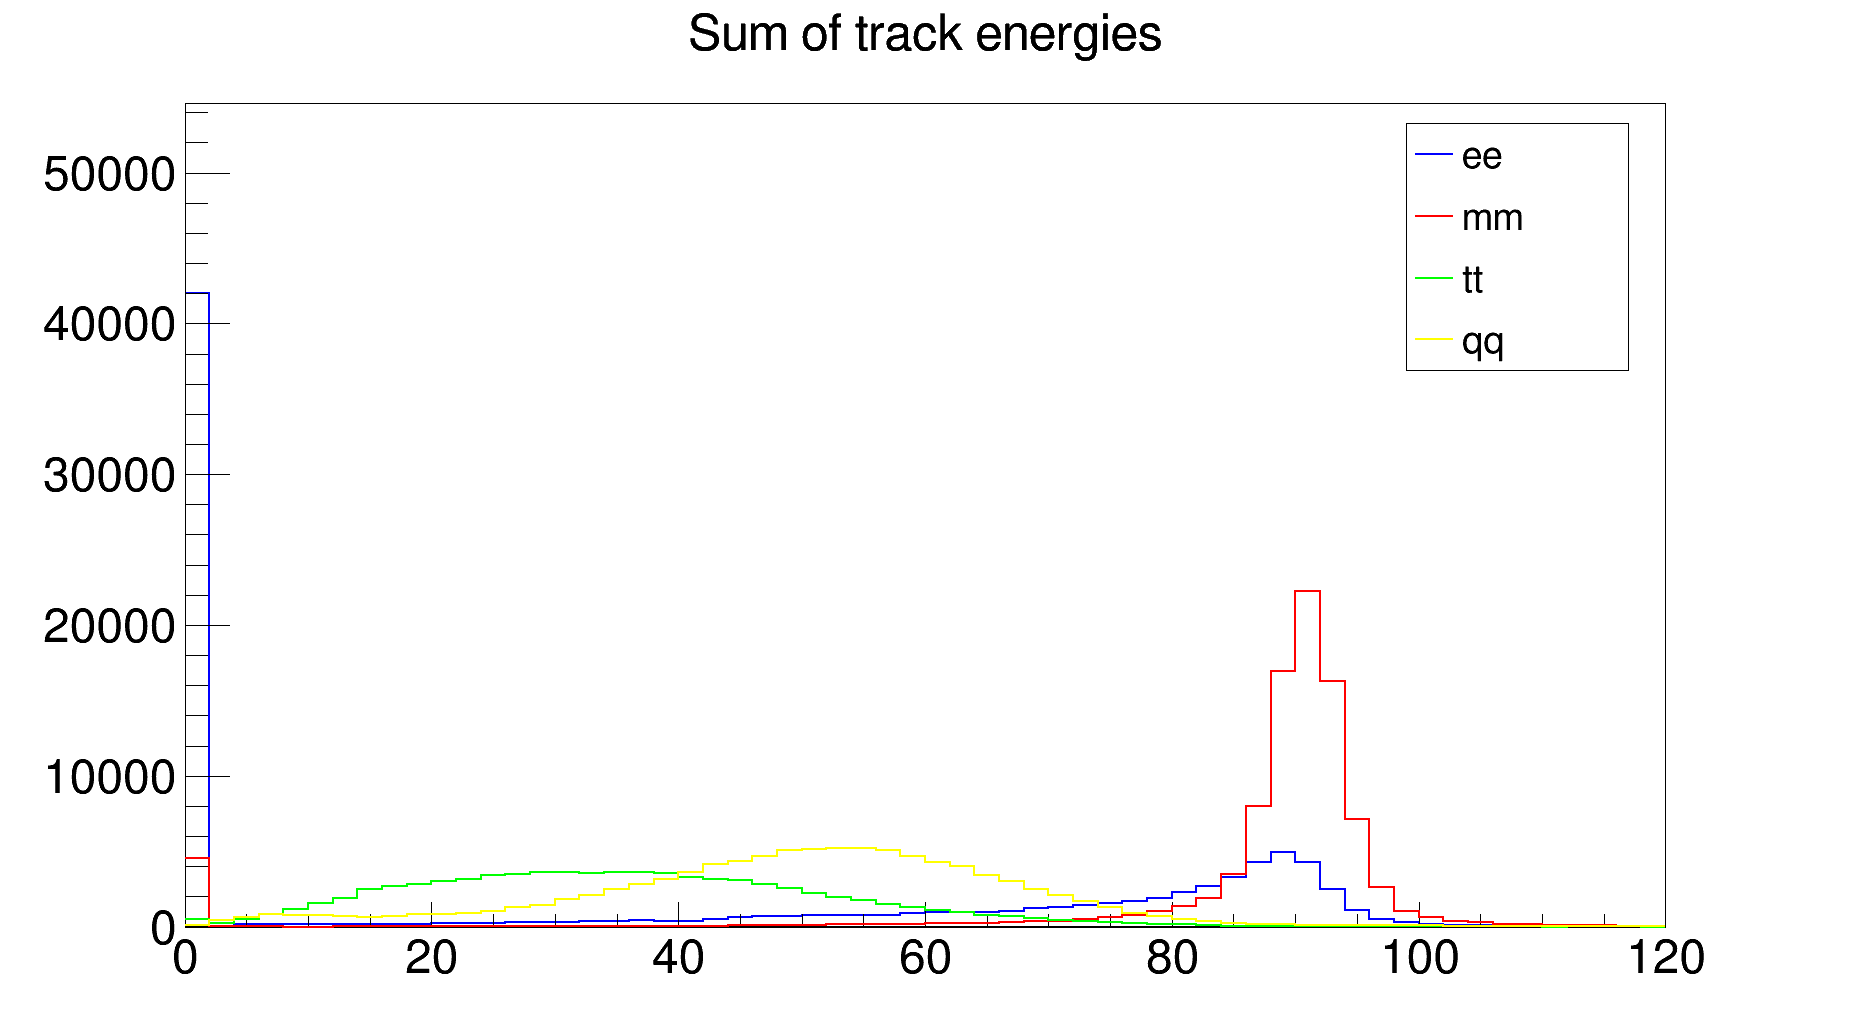
\includegraphics[width=1\linewidth]{../results/MC_results/nocut/Pcharged}
\caption[Pcharged in simulation data]{This figure shows the sum of track energies in the simulation data. }
\label{fig:Pcharged}
\end{figure}

\subsection{Cuts in Pcharged}
The separation of the data sets is less obvious in the Pcharged channel. Most datasets overlap, preventing the very clean cuts as they were in the Ncharged channel.


\begin{figure}[h]
\centering
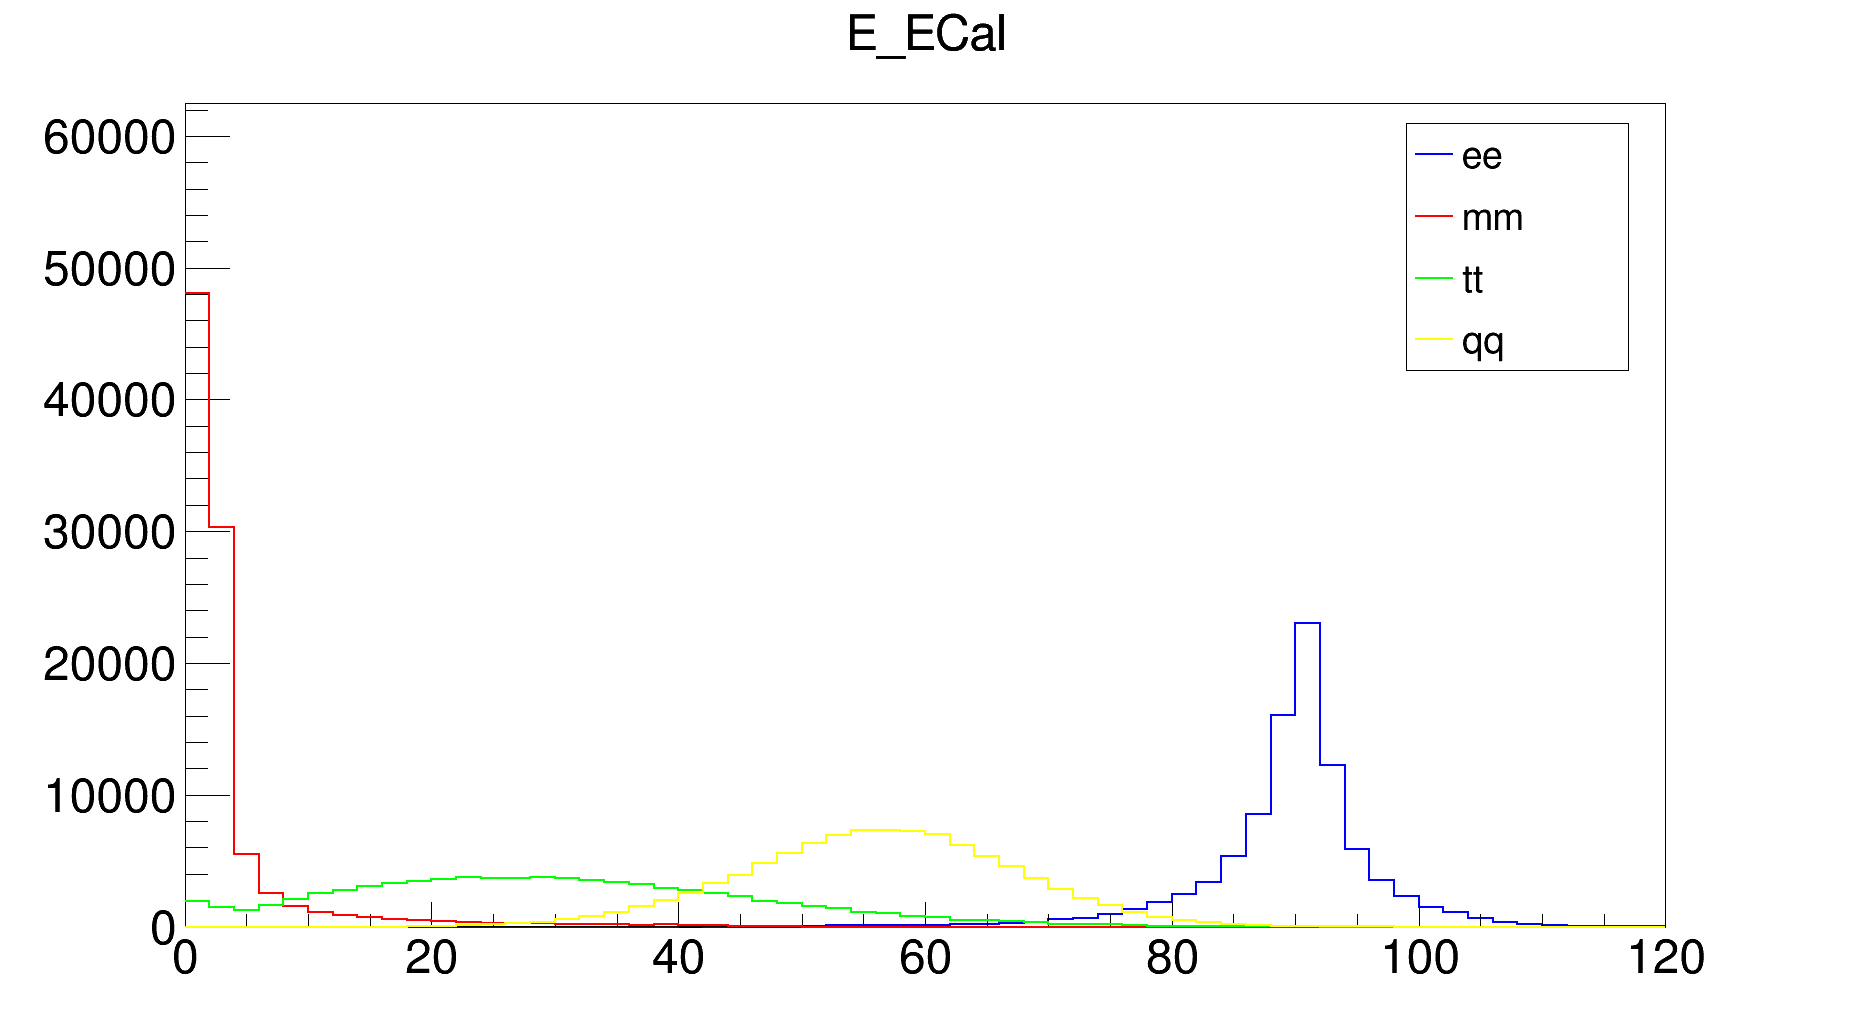
\includegraphics[width=1\linewidth]{../results/MC_results/nocut/E_Ecal}
\caption[E\_Ecal in simulations]{asd}
\label{fig:E_Ecal}
\end{figure}


\begin{figure}[h]
\centering
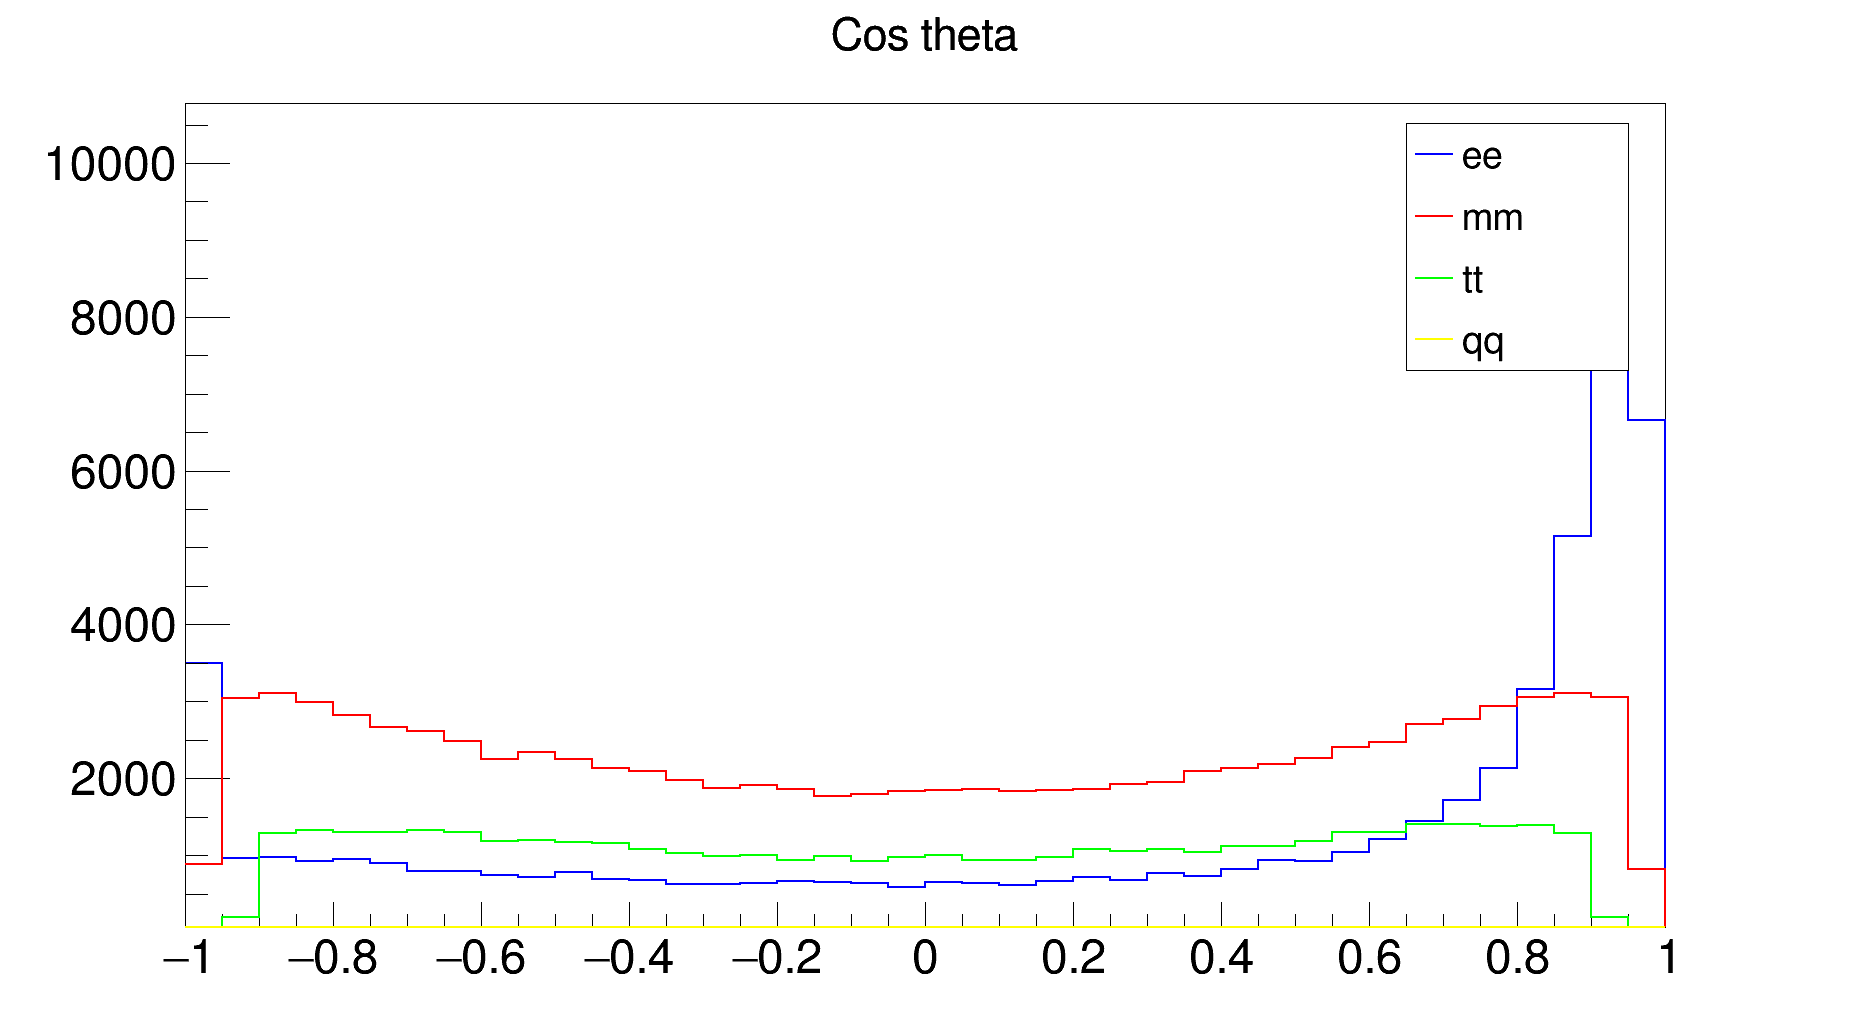
\includegraphics[width=1\linewidth]{../results/MC_results/nocut/cos_theta}
\caption[Cos\_theta in simulation data]{This figure shows the cosine of the angle between the beam and the direction of the created anti-lepton. Note the asymmetric peaks in the electron data, which will be discussed in the chapter on the separation of s- and t-channel.}
\label{fig:cos_theta}
\end{figure}

\subsection{Cuts in Cos\_theta}
MENTION NON EXISTING QUARKS DATA


\begin{figure}[h]
\centering
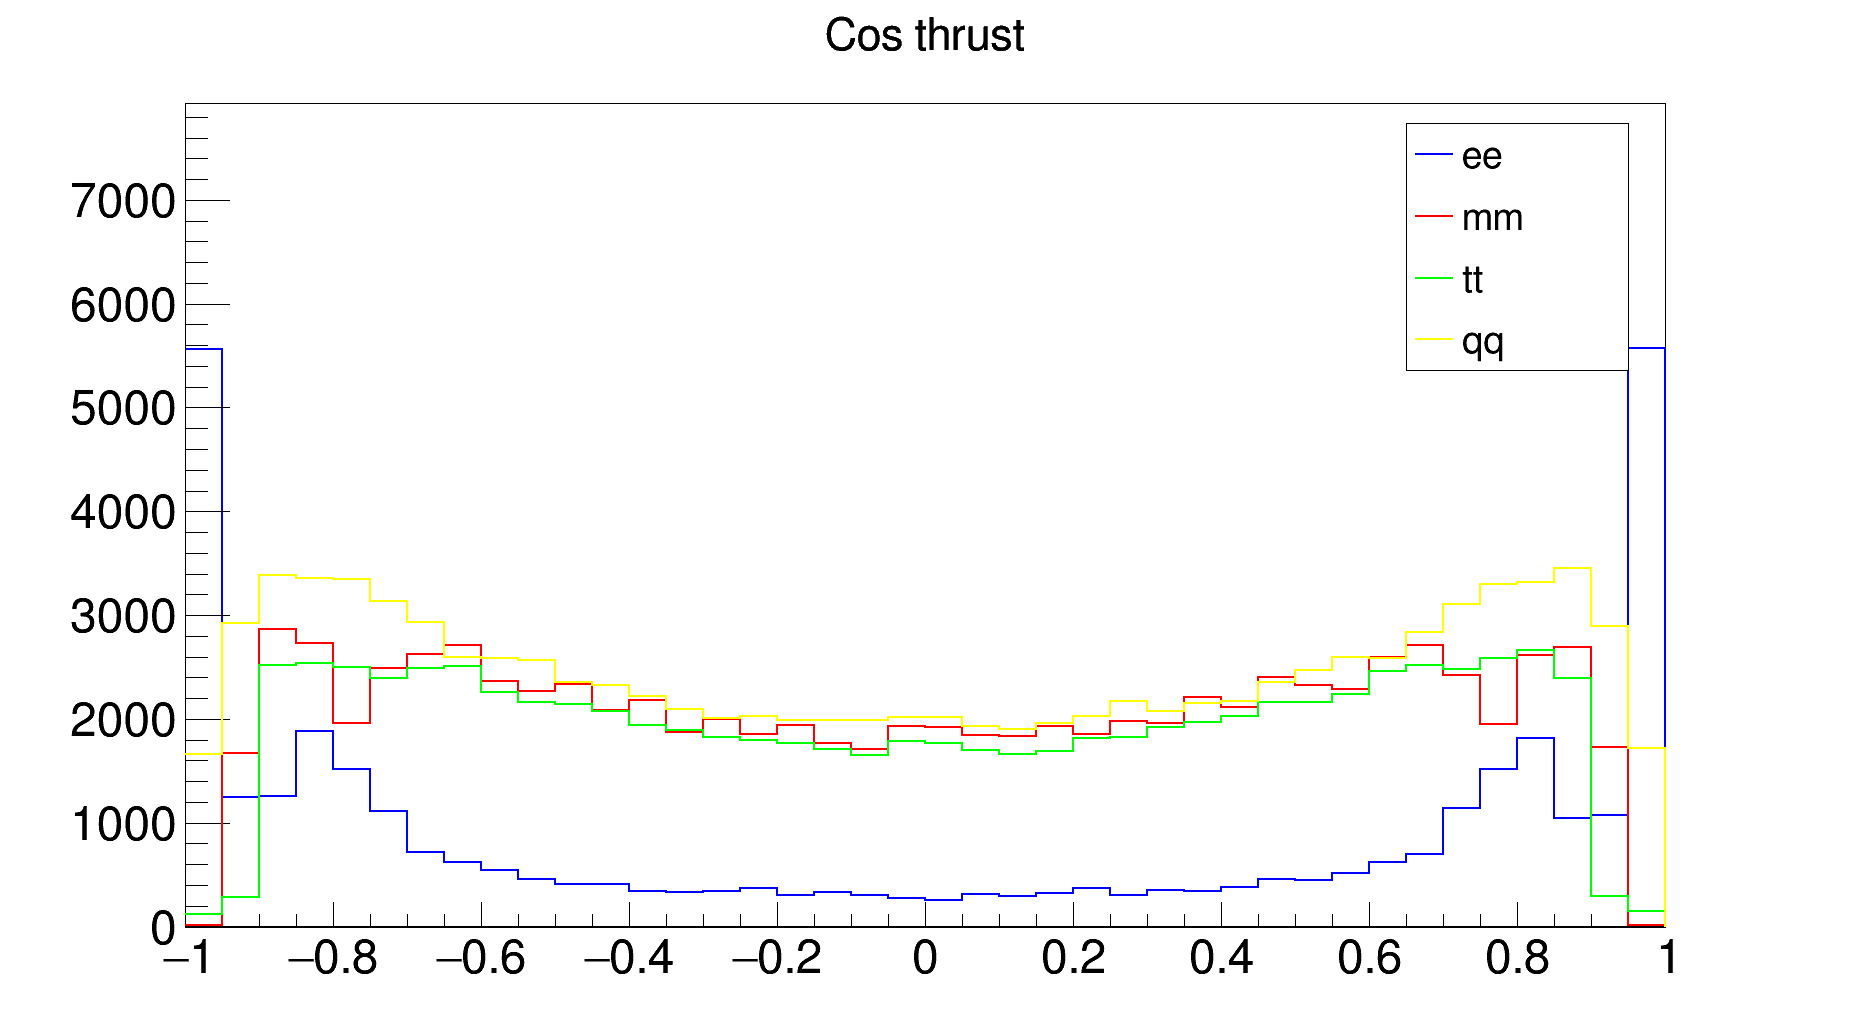
\includegraphics[width=1\linewidth]{../results/MC_results/nocut/cos_thru}
\caption[Cos\_thru in simulation data]{This figure shows the cosine of the angle between the beam and the thrust direction.}
\label{fig:cos_thru}
\end{figure}

\subsection{Cuts in Cos\_thrust}




